

\subsection{Schematic diagram of the actuator control device}

The schematic diagram of the actuator control device for the mini manipulator robot is shown in Figure \ref{PACD}. Microcontroller U9 is the main computational component of the actuator control system. The STM32G431CBU6 chip is connected according to the standard scheme from the datasheet \citep{STM32G431}. The DC-DC converter is the main power source for the entire actuator control device, and the microcontroller works with an analog signal. To improve the stability of analog operational amplifiers and the accuracy of the ADC operation, a noise suppression filter on the analog power line VDDA and the reference voltage line VREF+ is implemented in the circuit, assembled according to the notes in AN5346 \citep{STM2019}. The microcontroller is clocked using quartz resonators X1 and X2, which are connected according to the standard scheme with capacitors C23, C24 for X1 and C18, C19 for quartz resonator X2. Quartz resonator X1 serves as the main generator of the 8 MHz HSE clock signal for microcontroller U9. Quartz resonator X2 has a specific low-speed frequency LSE 32.768kHz, necessary for the real-time clock (RTC) operation, which is used for precise timekeeping without accumulating errors in the case of binary conversion. For programming the microcontroller, the programmer-debugger pins are led out to connector H2.

To monitor the state of the actuator device, two LEDs, LED1 and LED2, are provided. LED1 is connected through a current-limiting resistor to the power supply and lights up when power is applied, while LED2 lights up when needed from the MCU signal and serves as an indicator of the actuator device's error. An input voltage divider, consisting of resistors R16 and R18, is connected to the ADC input PA0 of the microcontroller; the resistance values are chosen to be more than 10 kOhm to prevent a large voltage drop across the resistors, with a maximum measurable voltage of 3,3 Volts. The second ADC input PB14 is connected to the outputs of the temperature measurement circuit, consisting of NTC resistor R15 and balancing resistance R20; capacitor C30 serves as a low-purity filter element with an upper boundary frequency of 1.5 kHz.

\begin{figure}[H]
	\begin{adjustbox}{addcode={\begin{minipage}{\width}}{\caption{
						Schematic diagram of the actuator control device
						} \label{PACD}
					\end{minipage}},rotate=90,center}
		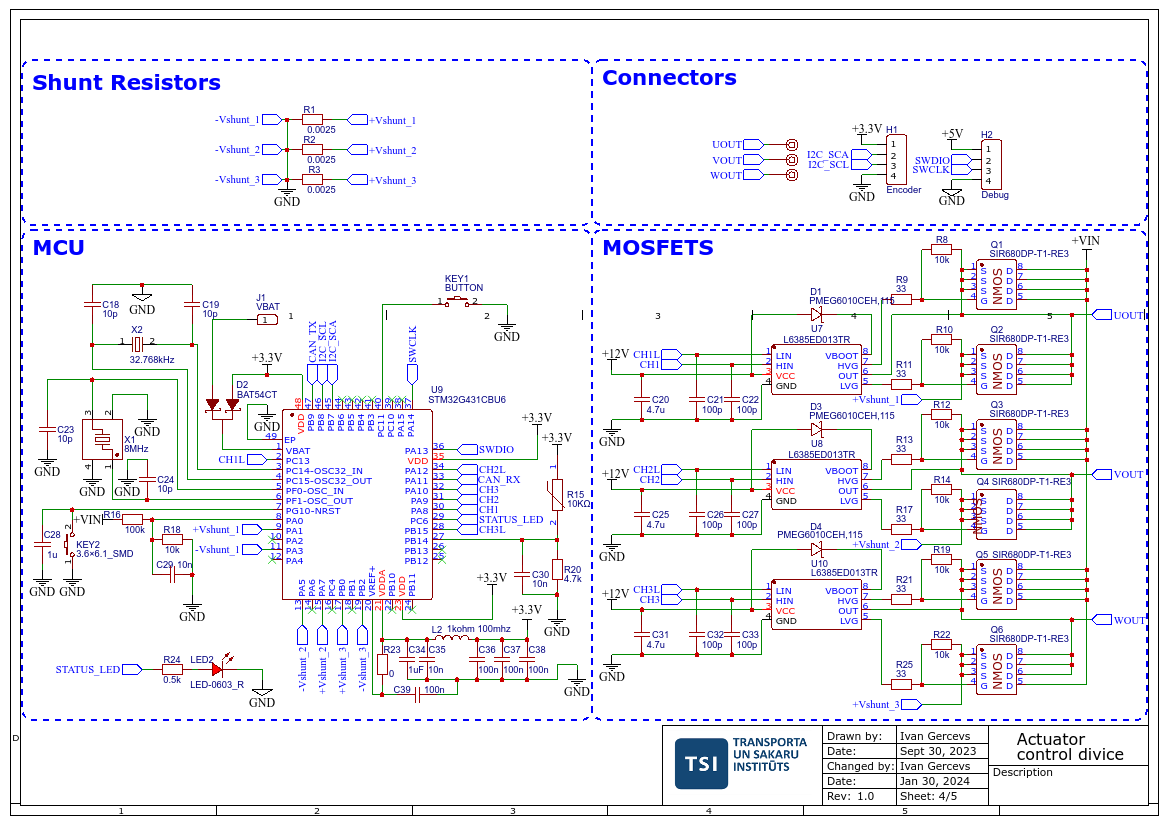
\includegraphics[width=0.85\paperheight]{Src/images/ACD.png}
	\end{adjustbox}
\end{figure}

Inverter drivers U7, U8, U10 are connected to the output of timer TIM1, located on the lines of port A and C. To suppress high-frequency interferences, capacitors C21, C22, C26, C27, C32, C33 with a value of 100 picofarads are connected to each of the inputs. Capacitors C20, C25, C31 on the power line are installed to prevent a sharp voltage drop when the internal power transistors are opened. Diodes D1, D3, D4 form a startup load circuit, necessary to provide power to the high-voltage section of the driver. The drivers control the power transistors from Q1 to Q6; the half-bridge driver controls the upper and lower level transistors for each motor phase. The transistors are connected through low-resistance resistors R9, R11, R13, R17, R21, R25 to eliminate ringing (parasitic oscillation) and through resistors R8, R10, R12, R14, R19, R22, which pull the gate to the source to avoid parasitic openings of the transistors.

For data bus communication, MCU lines PB9 and PA11 are connected to the CAN BUS transmitter U4, as shown in the schematic diagram \ref{PPACD}. The transmitter does not require a standby mode, so the STB pin (pin 8 of the chip) is connected to the ground, and the transmitter operates from the moment it is turned on. A terminal resistor R7 is provided between the CANH and CANL lines, connected via jumper H3. For easy installation of executive control devices, connectors JP2 and JP1 form a parallel connection of two connectors, allowing the connection of devices without creating additional connections on the wires. The power connectors CN1 and CN2 are connected using the same principle.

This device implements several options for voltage and current conversion. The main converter is the DC-DC converter chip AP64502QSP, which is connected according to the standard scheme from the datasheet, as shown in the schematic diagram \ref{PPACD}.

The chip converts the input voltage to the required 12V voltage for powering the power transistor drivers. To ensure voltage conversion, it was necessary to calculate the feedback divider at the FB (Feedback) line input, which is calculated (\ref{R4}):
\begin{ceqn}
	\begin{align} \label{R4}
		R4=R6\cdot(\frac{V_{out}}{0.8V}-1)
	\end{align}
\end{ceqn}
where R2=10 kOhm, for this variant the values are R1=140 kOhm. Capacitor C6 on the SS line of the DC-DC converter is a soft-start time setter. The standard variant 10nF was chosen, which is approximately equal to the soft start time - 4 ms\citep{AP64502Q}.

\begin{figure}[H]
	\begin{adjustbox}{addcode={\begin{minipage}{\width}}{\caption{
						Schematic diagram of power supply elements and data bus of the actuator control system
						} \label{PPACD}
					\end{minipage}},rotate=90,center}
		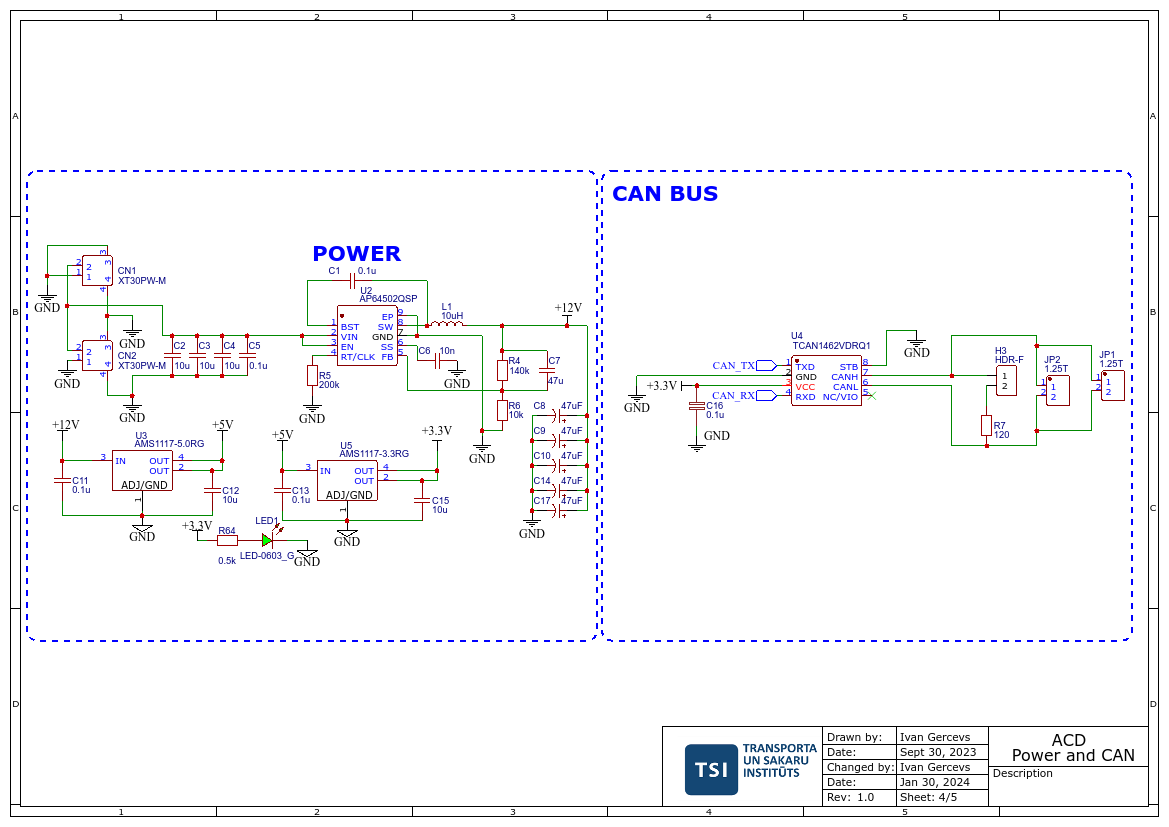
\includegraphics[width=0.85\paperheight]{Src/images/ACD POO.png}
	\end{adjustbox}
\end{figure}

The coil inductance is calculated for this inverter using the formula (\ref{L}), where Delta $I_{l}$ for this connection is calculated using the formula (\ref{Il}):
\begin{ceqn}
	\begin{align} \label{L}
		L = \frac{V_{out}\cdot(V_{in}-V{out})}{V_{in}\cdot\Delta  I_l\cdot f_{sw}}
	\end{align}
\end{ceqn}

\begin{ceqn}
	\begin{align} \label{Il}
		\Delta I_l = 0.5 \cdot 5A
	\end{align}
\end{ceqn}

The chip has a frequency control from 100kHz to 2.2MHz, the frequency is set by the resistor R5, the frequency is calculated by the formula (R5):
\begin{ceqn}
	\begin{align} \label{R5}
		R5 = \frac{100000}{f_{sw}[kHz]}
	\end{align}
\end{ceqn}

For the conversion option, the closest in parameters inductance L = 10 μH \citep{AP64502Q} was chosen. An additional row of smoothing tantalum capacitors C8, C9, C10, C14, C17 has been introduced into the standard converter scheme. Tantalum capacitors have a low internal resistance (ESR), which affects the output ripple (\ref{Vr}):

\begin{ceqn}
	\begin{align} \label{Vr}
		V_{outRipple} = \Delta I_l \cdot (ESR + \frac{1}{8\cdot f_{sw} \cdot C_{cout}})
	\end{align}
\end{ceqn}

The total capacitance of the capacitors is $5 \times 47\mu F$.

Linear voltage converters U3 and U5 are used for voltage conversion for microcontrollers. The linear converters are connected to the 12V power line to reduce the heating of the converters themselves by reducing the voltage drop across them.

Torque measurement is carried out by measuring the current of the electric motor. The voltage drop across the shunts is measured, shunts R1, R2, and R3 have very low resistance to avoid the influence of the transmitted voltage and excessive heating. The shunt outputs are connected to the microcontroller inputs. After configuring the microcontroller, the shunt input lines are connected to the internal operational amplifiers and used in further conversions.

 
\subsection{ Schematic diagram of the tactical control device}
The Shematic diagram of the tactical control system of the mini robot manipulator device is shown in Figure \ref{PPTCD}.

\begin{figure}[H]
	\begin{adjustbox}{addcode={\begin{minipage}{\width}}{\caption{
						Schematic diagram of the tactical control device for minirobot manipulator
						} \label{PPTCD}
					\end{minipage}},rotate=90,center}
		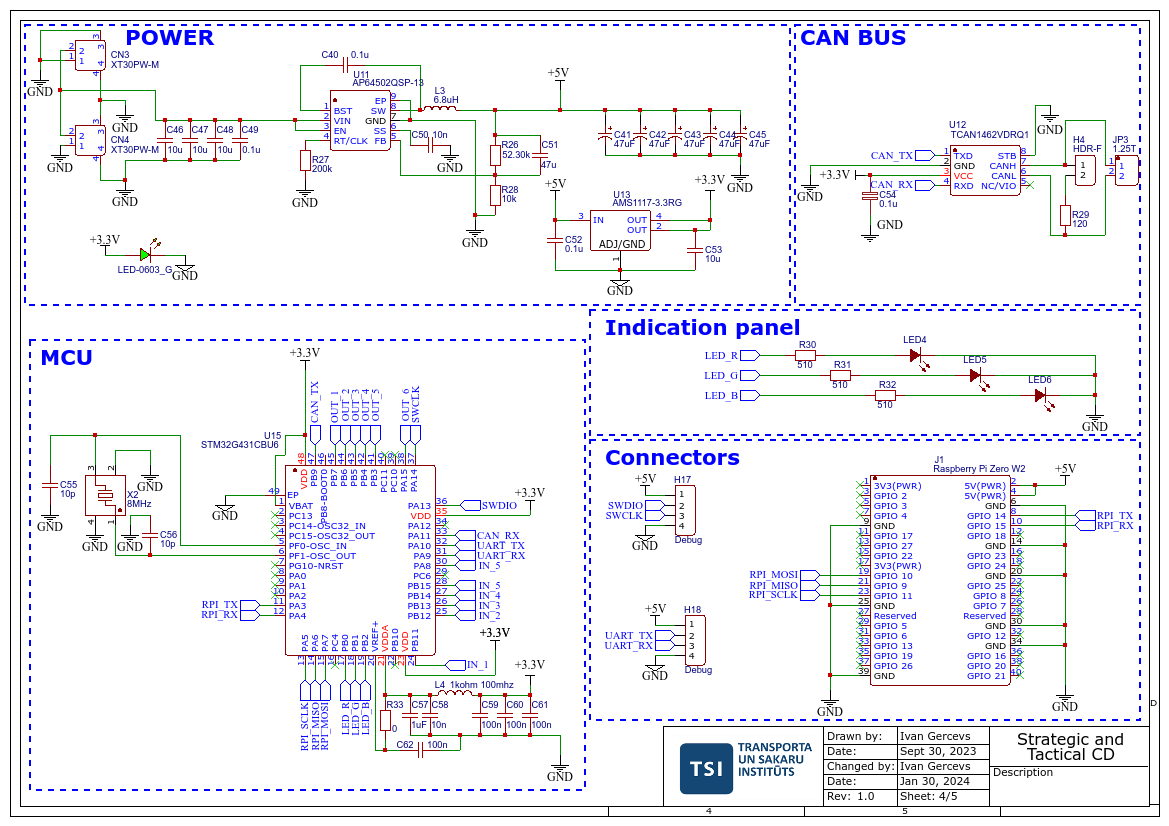
\includegraphics[width=0.85\paperheight]{Src/images/TCD.png}
	\end{adjustbox}
\end{figure}

\begin{figure}[H]
	\begin{adjustbox}{addcode={\begin{minipage}{\width}}{\caption{
		S				Schematic diagram of the pin inputs for the control system of a mini-robot manipulator
						} \label{DI_DOTCD}
					\end{minipage}},rotate=90,center}
		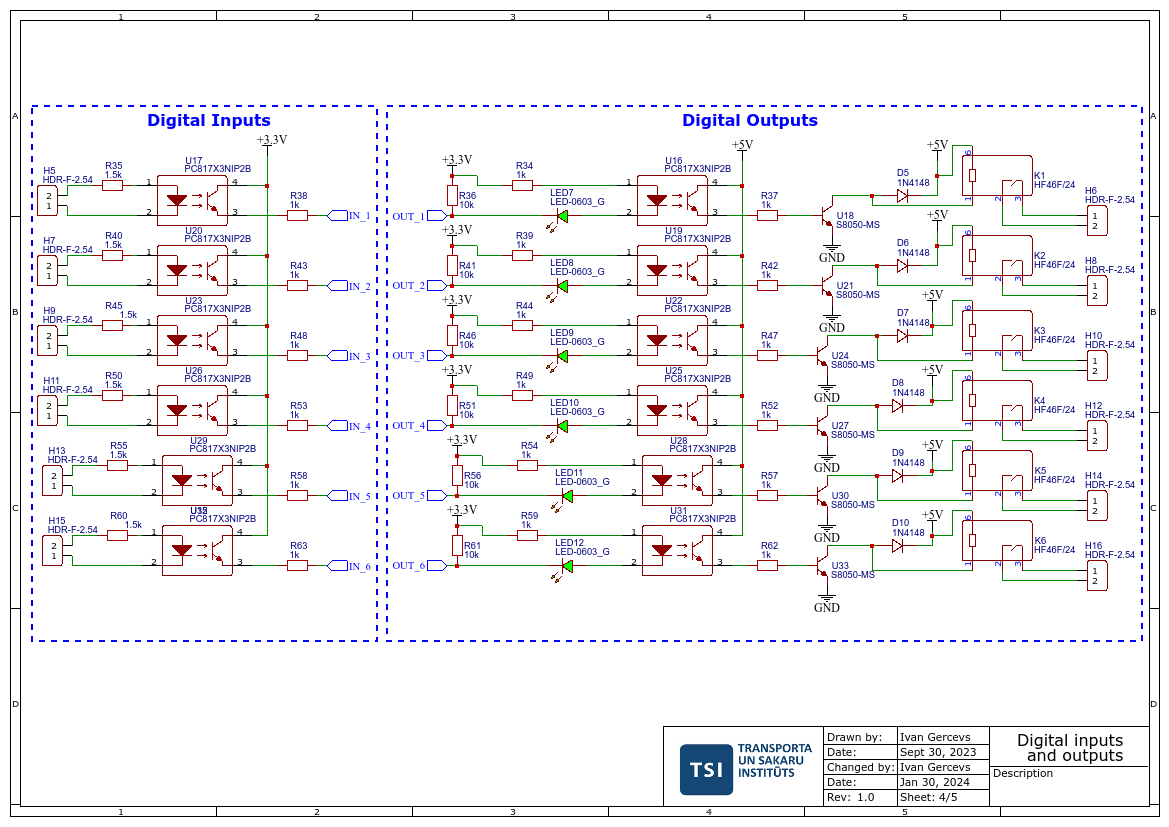
\includegraphics[width=0.85\paperheight]{Src/images/Di_DO.png}
	\end{adjustbox}
\end{figure}

The microcontroller U15 is a tactical control device assembled according to a standard scheme, as shown in the figure \ref{PACD}. The strategic control device connects through the J1 connector and utilizes two interface options: SPI and UART. The other pins of the J1 connector are not used, as they can connect to various expansion boards for the "Raspberry PI ZERO 2", which expand the functionality of the single-board computer.

The indicator panel consists of three LEDs of 3 colors: LED4, LED5, LED6, and they are connected to the microcontroller input. The other free inputs and outputs of the microcontroller are divided for controlling external signal inputs (6 pieces) and outputs (6 pieces) and are connected according to the standard scheme from the datasheet.

The inputs and outputs are isolated using optocouplers, shown in the figure \ref{DI_DOTCD}, and the output signals are switched using relays K1, K2, K3, K4, K5, K6. The signals from the optocouplers U16, U19, U22, U25, U28, U31 are amplified by the transistors U18, U21, U24, U27, U30, U30. A resistor in the base circuit is necessary to limit the current flowing to the transistor's base. Diodes D5, D6, D7, D8, D9, D10 are needed to shunt the relay coil terminals when the power is turned off. When switching off, a back EMF (electromotive force of self-induction of the coil) pulse is generated at the coil terminals, and this pulse can reach tens of volts and can lead to the failure of transistors U18, U21, U24, U27, U30, U30, which are not designed for such voltage.

The input digital signals are isolated using U17, U20, U23, U26, U29, U32. It is assumed that a logical "1" corresponds to 24V voltage. To ensure the activation of the optocoupler, the resistors R35, R40, R45, R50, R60 were calculated with the condition that the current through the optodiode inside the optocoupler should be 20 mA at a voltage of 1.2 Volts, the maximum allowable voltage is 30 Volts, and the approximate resistor value was chosen from the E24 resistance value series and corresponds to 1.5 kOhm.